\section{Experiment}
\label{sec:experiment}
%\shuqing{Many parts in this section are much more likely to lie in implementation, introducing how \tool works. Doesn't look like experiment.}

%\shuqing{Experiment for devices and case study needed.}

To evaluate the effectiveness of \tool in different modes, we conducted three
experiments on \tool using devices with \ac{USB} Type-C capabilities from different
\acp{OEM}, including a mobile phone, a tablet, and a laptop.

\textbf{Setup.}
%\fengwei{I would suggest to add references for devices such as
%Pi, ATMEGA32U4 board, Yamazawa, etc.}
As mentioned in Section~\ref{sec:badusb},
our \tool only requires common components that are easily accessible online or
in any electronic store. Here we choose the following parts to build a
prototype. To begin with, we choose the Raspberry Pi 4B~\cite{pi4b} as the embedded Single Board
Computer inside \tool, which is powerful enough to process video data and has
an onboard WiFi chip. As for the \ac{HID} Emulator, we use an Atmel ATMEGA32U4 board~\cite{atmel}
with \ac{USB} protocol support, which is able to emulate multiple \acp{HID}
with our modified firmware. About the \ac{USB} 3.x Hub, we use one from the
UGREEN~\cite{ugreen}, which supports HDMI, \ac{USB} 2.0, and many other exported peripherals.
Apart from these essential parts, we also use an auxiliary power-bank to
provide power for the Raspberry Pi and the mobile devices used by the victim.
The image of our \tool prototype can be found in Figure~\ref{fig:armory}.

\circled[text=white,fill=myblue]{\scriptsize{A}} is a Huawei mobile phone, the victim's device; \circled[text=white,fill=myblue]{\scriptsize{B}} is a compact look of \tool prototype; \circled[text=white,fill=myblue]{\scriptsize{1}} is the \ac{USB} 3.x Hub; \circled[text=white,fill=myblue]{\scriptsize{2}} is a Raspberry Pi 4B as the Single Board Computer; \circled[text=white,fill=myblue]{\scriptsize{3}} is an auxiliary power bank; \circled[text=white,fill=myblue]{\scriptsize{4}} is the Video Capture Card; \circled[text=white,fill=myblue]{\scriptsize{5}} is an Atmel ATMEGA32U4 board as the \ac{HID} Emulator.
%\fengwei{We need to explain the Figure. What is "A"? What is "B", Where are 1,
%2, 3, 4, and 5?}\hongyi{Is the caption sufficient? If explain here, I feel quite redundant}
%\fengwei{I think it is necessary to explain them in the text again.}


\begin{figure}[t]
	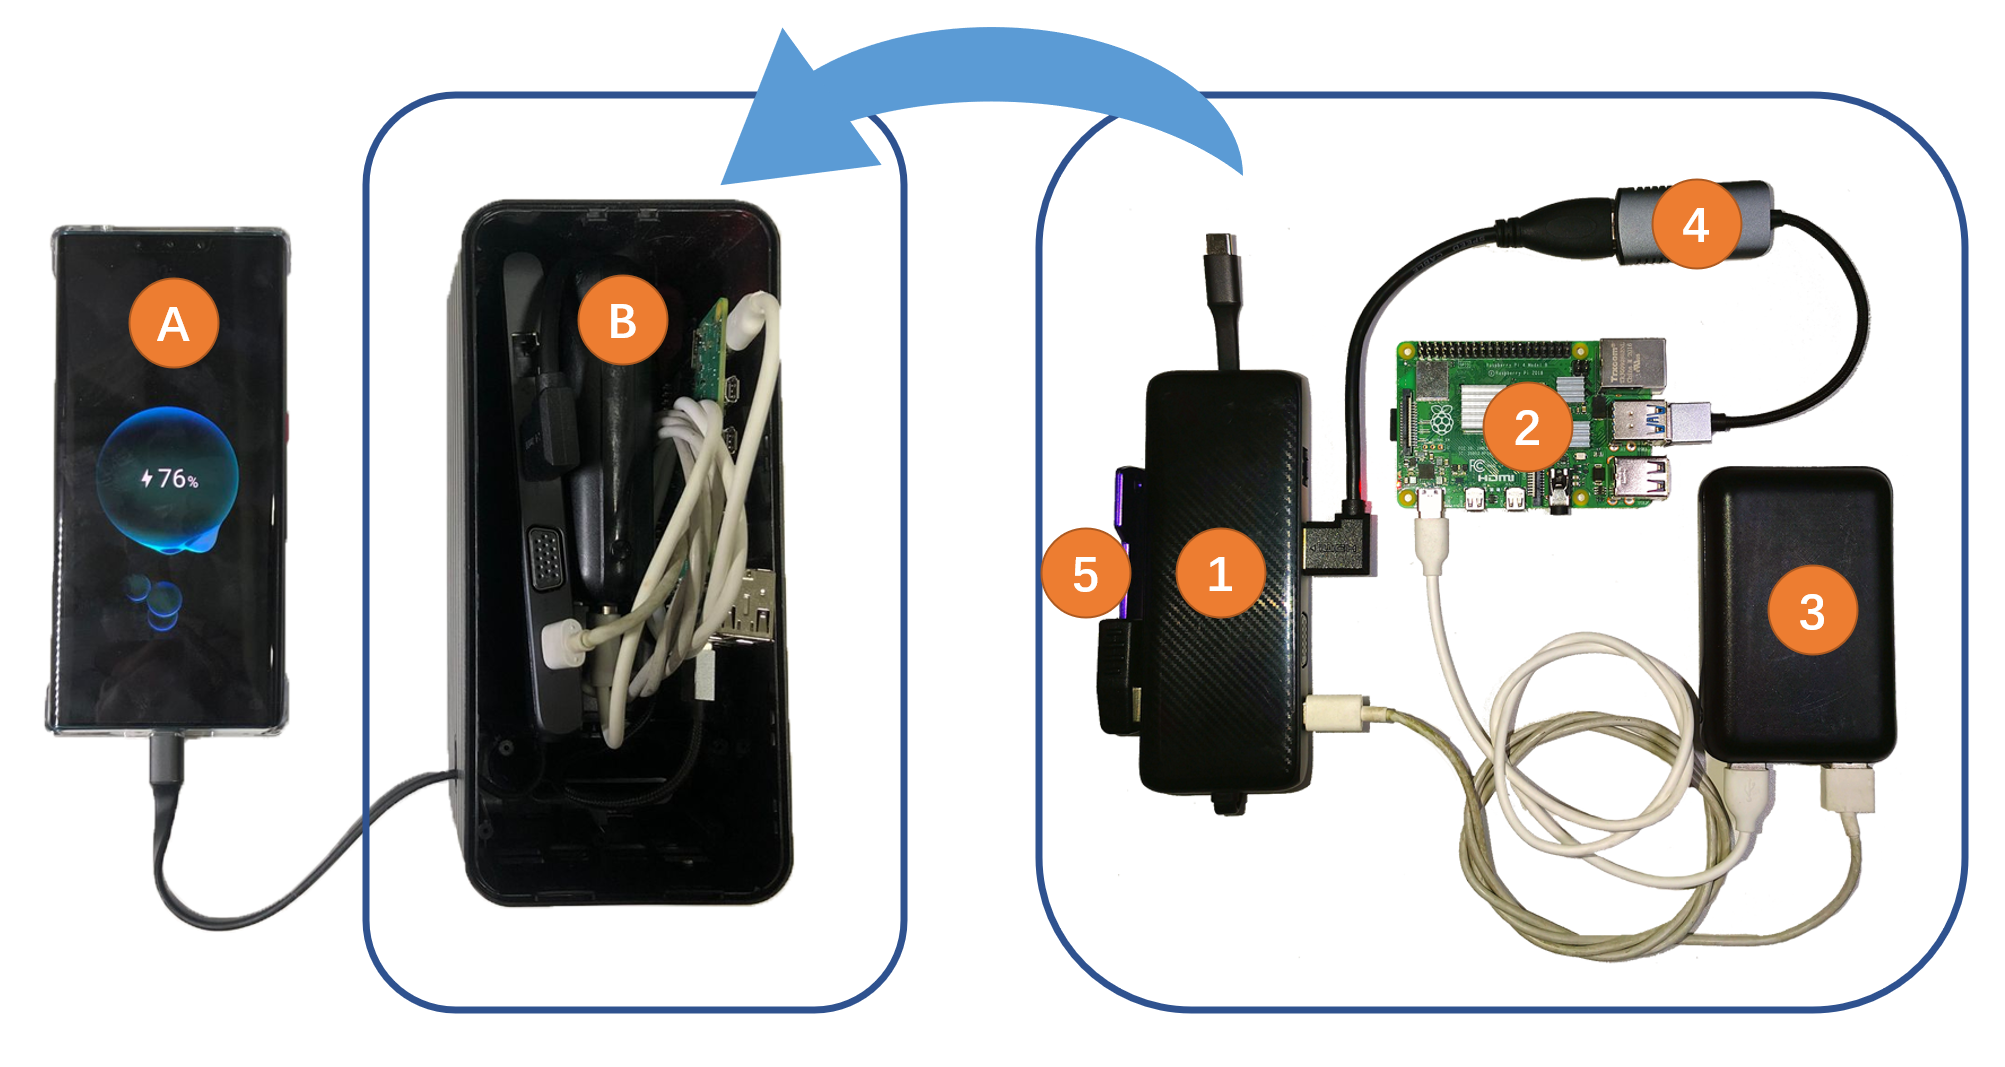
\includegraphics[width=\linewidth]{./Figs/armory_all.png}\\
	\begin{tabular}{ll}
	\circled[text=white,fill=myblue]{\scriptsize{A}} Victim's Device    &\circled[text=white,fill=myblue]{\scriptsize{B}}~\tool\\
	\circled[text=white,fill=myblue]{\footnotesize{1}} \ac{USB} 3.x Hub        &\circled[text=white,fill=myblue]{\footnotesize{2}} Raspberry Pi 4B\\
	\circled[text=white,fill=myblue]{\footnotesize{3}} Auxiliary Power Bank &\circled[text=white,fill=myblue]{\footnotesize{4}} Video Capture\\
	\circled[text=white,fill=myblue]{\footnotesize{5}} ATMEGAA32U4 Board
	\end{tabular}


	\caption{\tool Prototype.}
	\label{fig:armory}
\end{figure}

\subsection{Attack Initialization}
After the \tool is plugged into the victim's device, there is an initialization process to make sure the \tool is able to carry out subsequent attack.
\begin{itemize}
	\item \textbf{Screen Mirror}:
		During our experiment, we noticed that some devices do not mirror their screen to our \tool by default. In this case, \tool will inject a sequence of keystrokes and mouse movements to set the victim's device into mirror their screen. For example, in Windows 10, \tool can inject `Win+P' keystroke and a mouse click on the `Duplicate' option. However, as \tool is unable to obtain the screen during this process, this can only be performed blindly with a possibility of failure.
	\item \textbf{Dismiss Notification}:
		In our experiment, we found that some devices will notify the user the presence of an external screen. During our experiment, the following notifications are raised: 
		\begin{itemize}
		 \item On Lenovo Xiaoxin Pro 13, it raised a pop-up asking user to select the functionality of the external screen. 
		 \item On Huawei P30, it showed a status bar indicator and a persistent notification about the external monitor.
		 \item On iPad Pro (\nth{3} generation), it also showed a blue status bar indicator and a notification about \ac{USB} accessories if iPad is locked.
		\end{itemize}
		To avoid being discovered by the victim, \tool can inject keystrokes and mouse movement to dismiss some of these notifications. For example, in the first case, \tool is able to inject a sequence of mouse movements to set the screen at mirror mode to dismiss the pop-up.
\end{itemize}
\begin{comment}
\begin{table*}[]
	\begin{tabular}{|c|c|c|c|}
		\hline
		Device                                                               & Operating System                                                                                         & Notification              & Dismiss Action                                            \\ \hline
		\begin{tabular}[c]{@{}c@{}}Lenovo Xiaoxin Pro 13\\ 2020\end{tabular} & Windows 10 (OS Build 18363.1379)                                                                         & Pop-up                    & ``Win+P''-\textgreater{}Mouse click on `Duplicate' Option \\ \hline
		\multirow{2}{*}{HUAWEI P30 (ELE-AL00)}                               & \multirow{2}{*}{\begin{tabular}[c]{@{}c@{}}EMUI 11.0.0.135(C00E128R2P5)\\ Android 10 based\end{tabular}} & Status bar indicator      & N/A                                                       \\ \cline{3-4}
		&                                                                                                          & Persistent notifications  & N/A                                                       \\ \hline
		\multirow{2}{*}{iPad Pro (3rd generation)}                           & \multirow{2}{*}{iOS 14.4 (Build 18D52)}                                                                  & Status bar indicator      & N/A                                                       \\ \cline{3-4}
		&                                                                                                          & Pop-up (only when locked) & N/A                                                       \\ \hline
	\end{tabular}
	\linebreak
	\caption{Notifications about \tool}
	\label{tab:notification}
\end{table*}
\end{comment}

\subsection{HID Emulator Mode}

In the experiment of HID emulator mode, we used {Lenovo Xiaoxin Pro 13
2020}, a PC in Windows 10 (OS Build 18363.1379) with two \ac{USB} Type-C interfaces as the
target device. During this experiment, \tool disguised itself as a normal keyboard and an external screen as feedback channel. When first plugged in, the victim's devices raise a pop-up window asking victims what mode should new screen be set to. \tool immediately inject a sequence of mouse movement and click to set itself as a mirror to the primary monitor. Thus we have successfully completed the attack initialization. Then we tested three scripts, ranging from reverse shell backdoor to malware payload execution, all of which resulting in success. Compared to original BadUSB attacks like Rubber Ducky, our \tool can provide attacker real-time feedback which allows attacker to perform more accurate attack.
%This also warned us that we need more thorough defense against such BadUSB
%attack.


%\fengwei{do we need a reference for OCR?}
%\hongyi{we have discussed this and decide no need.}
\subsection{Video Capture Mode}

During the experiment of privacy extraction via our video capture mode, we chose \textit{HUAWEI P30 (ELE-AL00)}, a
smartphone in EMUI 11.0.0.135(C00E128R2P5) (Android 10.0 based) with a \ac{USB} Type-C interface, as the
target device.  In the privacy extraction experiment, \tool passively captured video
from the victim's device and used \textit{OpenCV} to identify the sensitive
information from the video stream.  When the victim viewed text or photos with
text, \tool used the techniques of \ac{OCR}  to
extract text from corresponding video frames. In this experiment, the attacker had
successfully extracted text like name, address, ID number, and other sensitive
personal information. We also tested the payment code extractor, which enables
an attacker to identify payment code in the video stream and perform transactions
without the password. As this is also a part of our case study, more details about
the extracted sensitive data can be found in Section~\ref{subsec:case_study} and
Table~\ref{table:information_extracted}.

%\fengwei{I don't understand the following sentence. Both modes need to capture
%the video stream. Don't understand why it is more power-efficient.}
%\hongyi{Reasonable, changed to other advantage}
Note that the video capture mode only needs to
process the victim's video stream locally, it does not need to transmit the real-time video back to the attacker, which is needed when the network connection between \tool and the attacker is not stable.
%This mode is useful when there is no stable network connection between \tool and the attacker.

\subsection{Fully Control Mode}
%\fengwei{In BadUSB-C section, remote control model is after privacy extraction mode.}

To test the capability of the full control mode, we chose iPad Pro (3rd
	generation), a tablet in iOS 14.4 (Build 18D52) with a \ac{USB} Type-C interface, as the target
device in this experiment.  Besides disguising as normal \acp{HID} like a
conventional BadUSB~\cite{badusb}, \tool also transmitted real-time video
stream from the target device to the attacker via WiFi.  After the connection
establishment, the attacker performed a series of actions to test the capability of
\tool. In the beginning, the attacker accessed the album application on the iPad and
obtained all the photos inside. After that, the attacker sent messages via victim's
account. At last, the attacker performed a transaction using the
financial application. All of these tests resulted in success.

Through this experiment, we have found that with video transmission and mouse
emulation, \tool extensively expanded the attack capability of BadUSB,
especially in mobile devices. In short, we have archived the complete hijack of the victim's
device in this experiment.

\subsection{Case study}
\label{subsec:case_study}
\tool can be used in various attack scenarios, ranging from mobile devices to PC devices.
For example, \tool can be attached to the power station, which provides USB 3 hubs, in the airport to perform attacks.
Most people charge their laptops or smartphones in the power station in emergency, with negligence of security.
In the following paragraphs, 

\subsubsection{Background}


\begin{table*}[t]
	\centering
	\begin{tabular}{|l|l|l|l|}
		\hline
		\textbf{Keyword} & \textbf{Text}                                                             & \textbf{Name}                                   & \textbf{Frame Number} \\ \hline
		username                          & X 8B cas.******.edu.cn Username: 11****18 Password:                                        & \textless{}user1\textgreater{} & 385                                    \\ \hline
		username                          & Login Weibo Login with SMS and verification code ...... +86 151****4587                    & \textless{}user5\textgreater{} & 1947                                   \\ \hline
		username                          & QQ 14*****50| Login with phone number New user registration 2345678 9 0                    & \textless{}user3\textgreater{} & 4308                                   \\ \hline
		username                          & connect to *** username h*****l Save account information Open VPN.....                     & \textless{}user6\textgreater{} & 7925                                   \\ \hline
		phone number                      & Login with phone number ...... +86 186****2483 |                                           & \textless{}user1\textgreater{} & 313                                    \\ \hline
		phone number                      & Log in with your mobile phone number. ...... mobile phone number 131****9310 & \textless{}user9\textgreater{} & 210                                    \\ \hline
		@                                 & contact email 30*******7G@qq.com, contact phone 027-88******                               & \textless{}user7\textgreater{} & 5324                                   \\ \hline
		@                                 & Account 73*****5@qq.com @qq.com @163.com @gmail.com 	......      & \textless{}user6\textgreater{} & 621                                    \\ \hline
	\end{tabular}
	\linebreak
	\caption{Examples of Searching \ac{OCR} Results with Keywords.}
	\label{tab:ocr_keyword_example}
\end{table*}

\begin{table*}[t]
	\centering
	\begin{tabular}{|c|c|c|c|c|c|c|}
		\hline
		\textbf{Keyword}                               & Account & Password & Phone number & Email & Username & Regexp for email~  \\
		\hline
		\textbf{Number of records containing keywords} & 680     & 1,596     & 1,510         & 164   & 522      & 78                 \\
		\hline
		\textbf{Total Number of Records} & \multicolumn{6}{c|}{4,172} \\
		\hline
	\end{tabular}
	\linebreak
	\caption{Privacy Extraction Result.}
	\label{table:information_extracted}
\end{table*}

We first introduce the technical background of our case study, sharing power
bank service and QR code payment.

\textbf{Sharing Power Bank}.  Sharing power banks provide users with short-term
rental of power banks.  The company deploys power bank stations in the city and
users can rent a power bank from any of the power bank stations, charge their
device on the trip, return the rented power bank to the near stations, and pay
the rental fee.

Power bank sharing is a popular service in Asia, power bank stations are deployed
in markets, stores, and even newsstands. For example, Figure~\ref{fig:PBS_products} are photos
of two power bank stations in China, which are taken outside of a supermarket. Brick~\cite{Brick} is also such a power bank sharing service provider from
Sweden. It provides power bank rental service all over Sweden and is planning on expanding its
service to entire Europe.
\begin{figure}[t]
	\centering
	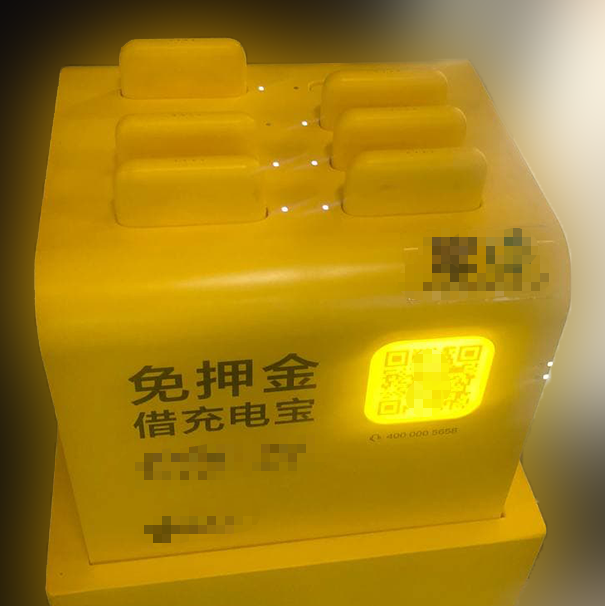
\includegraphics[width=.45 \linewidth, height=.45 \linewidth]{./Figs/PBS_mt.png}
	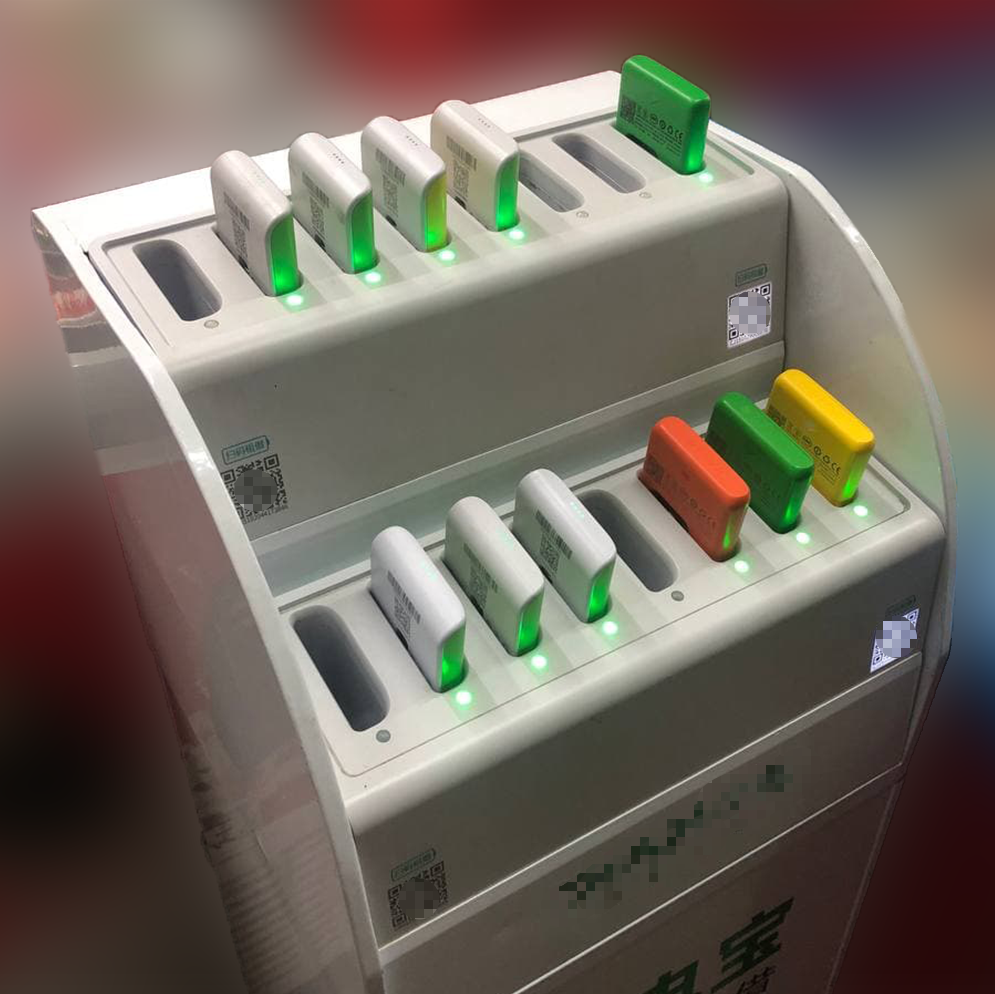
\includegraphics[width=.45 \linewidth, height=.45 \linewidth]{./Figs/PBS_xd.png}
	\caption{Two Power Bank Stations.}
	\label{fig:PBS_products}
\end{figure}

\shuqing{May use statistics (instead of concrete examples) to explain it.}

Not only do sharing power bank provide convenience to users, but it also
brings security issues.  We noticed that most of the power bank stations do not
check the integrity of power banks during the rental process, and users are
hardly cautious to check the power banks when connecting their devices.  An
attacker is able to tamper rented power banks and return them to a power bank
station causing a potential threat to subsequent users.


\textbf{QR Code Payment}.
QR code payment is a new type of payment method that is popular in Asia. Its most well-known cases are WeChat Pay~\cite{Wechat-pay} and Alipay~\cite{AliPay}. QR code payment provides merchant and client a convenient way of offline payment while ensuring equivalent security as the credit card.
As illustrated in Figure~\ref{fig:qr_payment_procedure}, QR code payment information from the video stream.  When the victim viewed text or photos withnt\shuqing{?} is typically performed in the following steps:
\ding{182} The client presents the payment QR code on the mobile device to the merchant.
The QR code is encoded with a globally unique ID to identify the client's account.
\ding{183} The merchant scans the payment QR code and charges the corresponding amount of money.
By presenting this QR code, the client authorizes the proceeding transaction.
\ding{184} After confirmation, the payment service provider proceeds with this transaction and returns the payment result to both the merchant and the client.
\shuqing{I think this paragraph can be shorter. No need to explain so many details.}
\hongyi{Dont know how to be more concise.}

\begin{figure}[t]
	\centering
	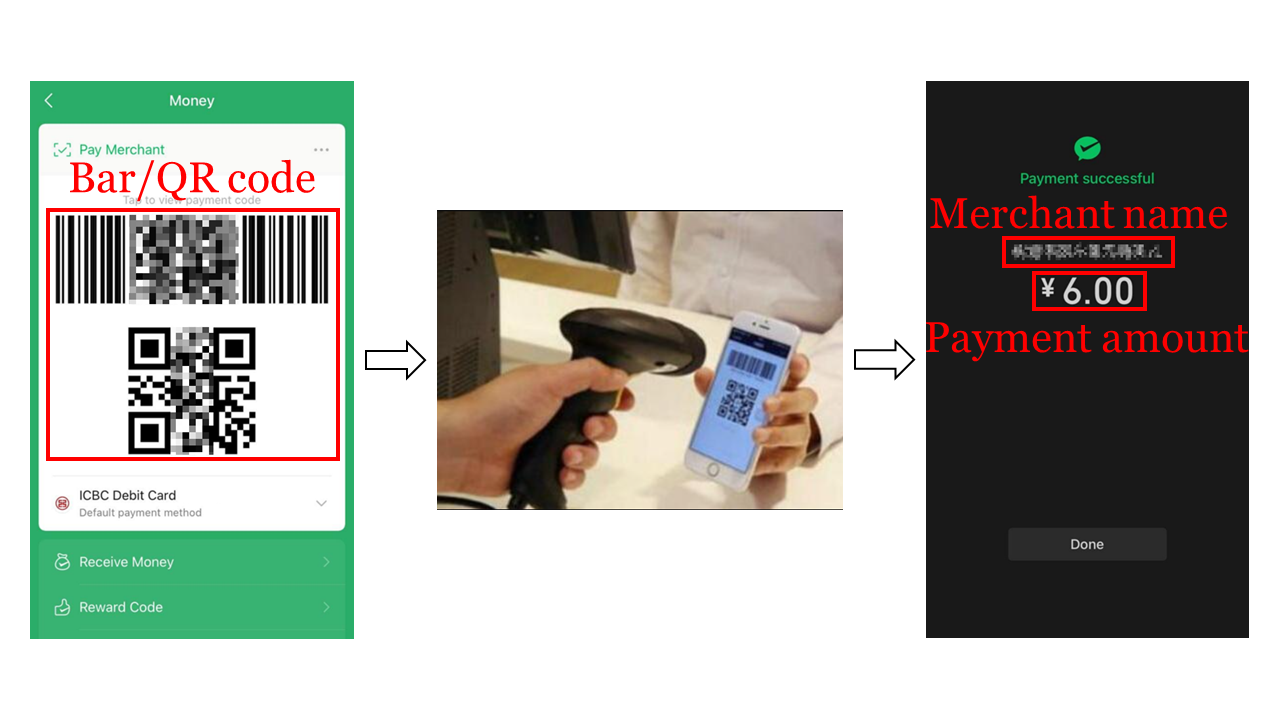
\includegraphics[width=\linewidth]{./Figs/qr_code_payment.png}
	\caption{Bar/QR Code Payment Procedure.}
	\label{fig:qr_payment_procedure}
\end{figure}


Next, we explain one type of payments called micropayment. A micropayment is pre-determined by the payment
service provider with thresholds in the user agreement. In real-world scenarios, payment service providers use different rules
for micropayment purchases. For example, WeChat
Pay~\cite{Wechat-pay} regards transactions under USD \textdollar 154 as
micropayments.  Different from a typical payment procedure, when micropayments
are made, confirmations can be applied automatically without clients'
permission which aims to provide convenience to both merchant and client.  If a
victim's payment code is leaked to the attackers, they can use that code to
authorize multiple micropayments without needing permission.  In order to prevent such
cases, both WeChat Pay~\cite{Wechat-pay} and Alipay~\cite{AliPay} have designed a refreshing mechanism for the
payment code, which is to refresh the QR code every minute. This is sufficient
to stop an attack like opportunistic theft of QR code but unable to stop a real-time attack like our
\tool.  In summary, the payment QR code is highly sensitive on users' devices
and our following case study is about how to obtain this code using an
attacker-crafted power bank via \tool.

\subsubsection{Attack Scenario}

In this part, we will introduce a real-life attack scenario to show that our
\tool is a practical offensive tool.  This scenario can be broken down into the
following steps.

\begin{enumerate}[I. ]
	\item The attacker rents a power bank from one of the power bank stations and replaces the internal components with \tool.
	\item After the modification, an attacker-crafted power bank is returned to a rental station in a crowded area like an airport or railway station, which increases the probability of success.
	\item A user borrows the modified power bank and connects it to her own device, becoming the victim of \tool.
	\item The attacker now has complete control over the victim and can perform various attacks using different modes.
\end{enumerate}

Next, we summarize the possible threats toward users under different modes.
%\hongyi{Better way to express this?}
First, under \ac{HID} emulator mode, the attacker is able to implant malware and backdoor script into victims' devices. Moreover, using video capture mode, once the victims accesses their sensitive data such as QR payment  code or photos, their sensitive data will be immediately transmitted via \tool to the attacker. Lastly, with full control mode, the attacker has complete control over the victims' device and can conduct any action on the victim device.

\shuqing{Background is longer than real user study.}
%As the functionality and effectiveness, HID emulator mode is similar to the original BadUSB and the full control mode hijacks the victim's device completely.
\hongyi{I dont know if it's a good enough reason}
%Here we only validate the usability of privacy extraction mode and conducted a user study.

To further validate our attacking scenario, we invited 10 volunteers, who are students in our university, to participate and conduct a user study.
Before the user study experiment, we discloses to the volunteers how their data might be used and request permission from the volunteers and the university ethics review boards.
During the case study, volunteers took turns to use their phones for half an hour with \tool connected, which is considered as a normal power bank usage time.
To obtain data close to real-life, they were requested to use phones just as they would when normally using the shared power banks.\shuqing{check}
After each experiment, the raw video and the corresponding \ac{OCR} result file will be generated automatically, then we presented these files to him/her, introduced our attack, told him/her to analyze the video file and replace certain characters of the private data that appear in the \ac{OCR} result file with asterisks. It protects their privacy and is also a mark for us to confirm that the data we find contains their private data. At last, he/she would destroy all original files, leave only the desensitized \ac{OCR} result for us. 
\shuqing{Do we need to mention that agreement the conference required here?}
\hongyi{I'm also quite concern about this.}


\subsubsection{Result}

After collecting the captured videos of the mobile phone, we analyzed the videos both automatically and manually.
During the automatic analysis, we used scripts to perform \ac{OCR} recognition for each frame in the recorded videos and stored all of the \ac{OCR} results in a database.
In total, there are 94,058 entries of data collected from 10 volunteers.
%\shuqing{The data may need to be updated.}
With these results, we could learn what content the victim visited, especially the privacy data.
%\fengwei{The following text needs to be revised. It is quite difficult for me to understand. Note that this is important text because reviewers are curious about the result. }
We searched the result database with the keywords \textit{account, username, password, phone number and email}, as well as the regular expression of email.
The records searched by such keywords and regular expression are usually related to privacy information of users.
For example, when we searched with \textit{account} as a keyword, victim's accounts can be found in the database, as shown in the Table~\ref{tab:ocr_keyword_example} and Table~\ref{table:information_extracted}.
%\shuqing{Statistics.}
The frame number is the position of this frame in the recorded video, which indicates a target for manual analysis for further data extraction.
At last, we found 4,172 of 94,058 records obtained by \tool which are related to privacy information, as shown in the Table~\ref{table:information_extracted}.


In the manual analysis, we replayed the videos and extracted sensitive information.
Accounts of internet applications such as Apple, iCloud, Facebook, Twitter can be obtained.
Moreover, all of the typing inputs on the virtual keyboard, including the system keyboard and the built-in security keyboards of the financial applications, can be clearly recorded.
We can obtain the plain text of passwords such as WiFi passwords.
Furthermore, the received SMS verification code (usually used to confirm real-name authentication) can be obtained when it appears in the top notification bar.

In summary, though we cannot directly obtain the user's password on the lock screen, we can still check all of the information presented on the screen, extract sensitive information including but not limited to social accounts, bank accounts, personal financial situation, etc., if the user unconsciously unlocks the screen.
It is worth mentioning that {secure keyboards} built in financial apps show their keyboard typing sequences, which can be easily captured by \tool.
